\chapter{本研究における課題定義と仮説}
\label{issue}

本章では,~\ref{background}章で述べた背景より,本研究における課題とその要件について議論し,先行研究および提案システムを概説することで本研究で用いるアプローチについて述べる.

\section{本研究における課題定義}
\label{issue:definition}

本研究では、惑星規模の分散システムのための試験環境の構築手法が整備されていないことを課題とする。

~\ref{bg:staging:planetary-scale-distributed-system}章で述べたように、惑星規模の分散システムは地理的に分散したコンピュータで構成されるため、ネットワーク上の通信の遅延がシステム全体に影響を及ぼす。
よって試験環境では、通信の遅延を考慮した上で地理的に分散したコンピュータの協調動作を試験しなければならない。
試験環境としてはPlanetLabやパブリッククラウドサービスの活用、BSafe.networkが既に知られているが、これらにはそれぞれ課題があると考える。
PlanetLabでは、世界中の717地域1353のサーバという地理的に幅広い選択肢が用意されているが、サーバのOSやCPU、メモリ等を柔軟に変更できない。
パブリッククラウドサービスでは、リージョンを活用することで地理的に離れた多数のデータセンターを利用することができるが、リージョンが限定的である。
BSafe.networkでは、世界中の32の大学が保有するサーバを用いてブロックチェーン技術に関する実験を行えるが、各サーバの管理権限が各大学のオペレータに委ねれていることで、
試験を行う際に各オペレータの手作業が必要となる。

\section{課題解決における要件}
\label{issue:requirements}

本節では,課題解決における要件を定義する.

~\ref{issue:definition}章で述べた課題を踏まえて、惑星規模の分散システムの試験環境の構築における必要要件は、
\begin{itemize}
  \item OSやCPU, Memoryといったサーバ環境を柔軟に変更可能であること
  \item 公の実稼働環境を想定したネットワークでの通信の遅延を考慮できること
  \item 異なる管理権限下にある各サーバに対し統合的管理が可能であり,各オペレータの手作業を軽減できること
  \item 地理的に分散した各サーバに対し,統合的な操作が可能であること
\end{itemize}
であると考えた。

\subsection{サーバ環境の柔軟性}
\label{issue:requirements1}

惑星規模の分散システムの試験では、OSやCPU、メモリ等のサーバの環境を柔軟に変更可能である必要がある。
何故なら惑星規模の分散システムにおいて、システムを構成するコンピュータの環境はユーザ依存であり開発者が一意に決めることはできないからである。
よって、異なるOSを搭載したコンピュータによる協調動作や、CPUやメモリといった資源を制限した場合の試験を行う必要がある。

\subsection{ネットワークでの通信の遅延の考慮}
\label{issue:requirements2}

惑星規模の分散システムは、地理的に分散したコンピュータによって構成される分散システムである。
そのため、各コンピュータが地理的に分散することによるネットワーク上の通信の遅延がシステムの動作に影響を与える可能性がある。
試験環境は、これらを考慮した上で試験が行える環境でなければならない。

\subsection{異なる組織間での試験における手作業の軽減}
\label{issue:requirements3}

BSafe.networkのように複数の組織間で惑星規模の分散システムの試験を行う場合、各サーバの管理権限が異なることにより、試験の遂行において各オペレータの手作業が必要となる。
各オペレータの手作業が要求されることによって、作業中の人為的ミスが発生する可能性が高まるとともに、手戻りによる作業の遅れが発生しやすくなる。
作業が各オペレータ依存になるため、サーバ構築における冪等性が担保されない問題もある。
試験環境では、属人的な手作業を軽減し試験が素早く正確に行わなければならない。

\subsection{地理的に分散したサーバの統合的な管理}
\label{issue:requirements4}

惑星規模の分散システムの試験環境では、すべてのサーバを統合管理する必要がある。
試験環境内のすべてのサーバに対し一斉に指示できるようにすることで、試験を迅速に進めることができるからである。
なお惑星規模の分散システムでは各サーバが地理的に分散しており、ネットワーク上で別のセグメントに配置されている可能性がある。
よって、試験環境では異なるセグメントに配置されたサーバに対して統合的な管理を行う必要がある。

\section{先行研究}
\label{issue:previous-research}

本節では、惑星規模の分散システムの試験環境の構築手法として提案された先行研究について述べる。
先行研究では、各コンピュータを操作するためのデバッグエージェントを独自実装したものや、ネットワークエミュレータを用いた仮想ネットワークによる手法が提案されている。
本研究ならびにPlanetLab、パブリッククラウドサービス、BSafe.networkでは実際に地理的に分散したコンピュータを用いているのに対し、
Emulabでは仮想的にネットワークを再現することで惑星規模の分散システムの試験を可能としている。

\subsection{P2Pアプリケーションの開発と性能評価のための統合開発環境の提案}

既存の提案手法として,地理的に分散したコンピュータを統合管理するためにデバッグエージェントと呼ばれる遠隔操作用のアプリケーションを独自で実装したものがある。
デバッグエージェントは,試験対象のアプリケーションに対して命令を送信したり通信内容をログとして抽出する。
デバッグエージェントを通して、P2Pアプリケーションの開発、性能評価を支援するための統合開発環境の構築に成功している。
しかし、デバッグエージェントは予め各サーバで動作させる必要がある。
また、デバッグエージェントは試験対象のアプリケーションに依存するため、アプリケーションの変更をする場合はデバッグエージェントにも修正が必要になる。

\subsection{プロセスレベルの仮想化を用いた大規模分散システムテストベッド}
\label{consideration:related-works:emulab}

分散システムや分散ネットワークを,ネットワークエミュレータによって構築された仮想的なネットワーク上で開発する取り組みである。
仮想ネットワークの構築にはEmulab~\cite{Emulab}を活用している。
Emulabは大規模なソフトウェアシステムであり,仮想ネットワーク内に点在するマシン同士の接続環境を自由に設定することが可能である.
数台のコンピュター上に数千台の仮想環境をプロセスレベルで構築し,それらをネットワークシミュレータにより相互接続することによって,擬似的なネットワーク環境における試験を可能にするものである.

\section{本研究における仮説}
\label{issue:hypothesis}

本研究では~\ref{issue:requirements}章で述べた実際性,統合性,拡張性を担保しながら地理的に分散したシステムのためのステージング環境を構築したい.
そこで,OpenVPNとKubernetesを活用することで,それらの要件を満たしたシステムが構築できるのではないだろうかと考えた.
それぞれの要件に対して,本研究で提案するシステムによる実現が可能であると考えられる点を本節では述べる.

\subsection{サーバ環境の柔軟性}
\label{issue:requirements1}


\subsection{ネットワークでの通信の遅延の考慮}
\label{issue:requirements2}


\subsection{異なる組織間での試験における手作業の軽減}
\label{issue:requirements3}


\subsection{地理的に分散したサーバの統合的な管理}
\label{issue:requirements4}

\section{提案システム概要}
\label{issue:about-system}

提案システムの概要を述べる.ステージング環境においてP2Pシステムに参加するノード同士を,OpenVPNを利用することで相互に疎通可能な状態にする.
OpenVPNオーバーレイネットワーク上でKubernetesクラスタを構築し,全てのノードをクラスタに参加させる.Kubernetesクラスタ内のマスターノードを
介して,全てのノードに対して操作を行うことができる.

\begin{figure}[htbp]
  \begin{center}
    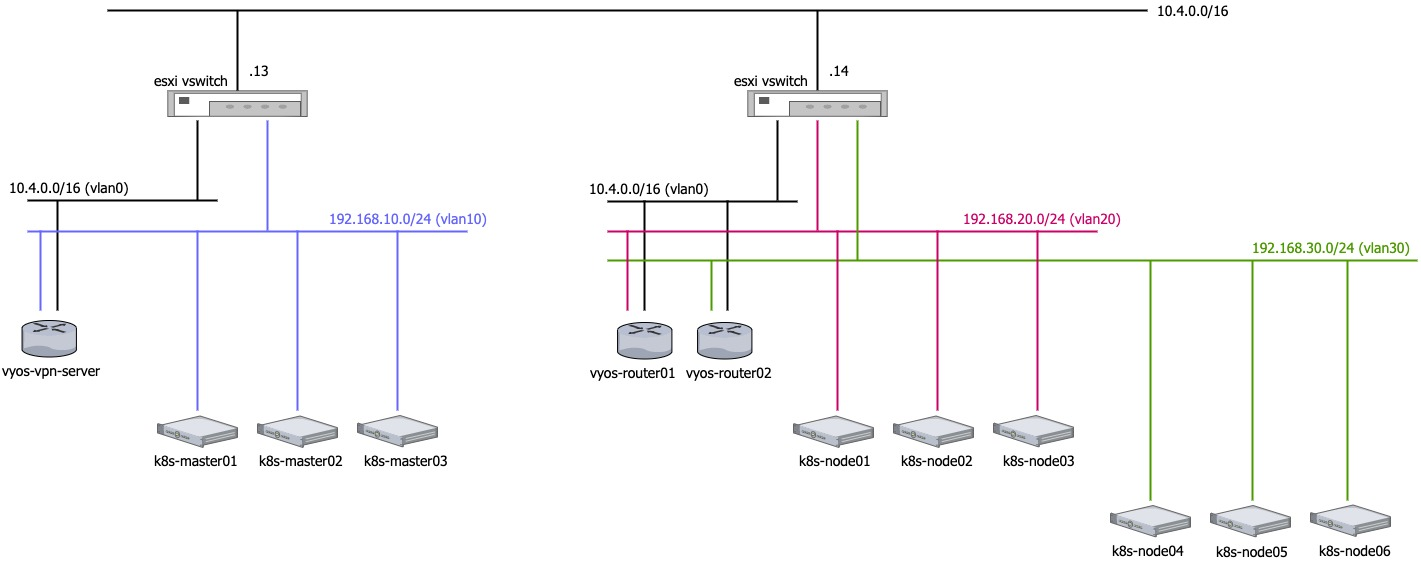
\includegraphics[width=\textwidth]{./figures/system-diagram.jpg}
    \caption{システム概要図}
  \end{center}
\end{figure}

%%% Local Variables:
%%% mode: japanese-latex
%%% TeX-master: "./thesis"
%%% End:
